%----------------------------------
% Review of Calc I and II topics.
%----------------------------------

%Note to Instructors: The matrix review section is commented with 'bmw' if-statement. In the Valpo version it has been moved to the Vector's unit.
\instructor{Note to Instructors: The matrix review section is commented with 'bmw' if-statement. In the Valpo version it has been moved to the Vector's unit.}

When you complete this \chpname you should be able to:
\begin{enumerate}
\item Summarize the ideas you learned in Calculus I and II \valposhort{Math 131 and 132}, including graphing, derivatives (product, quotient, power, chain, trig, exponential, and logarithm rules), and integration ($u$-sub and integration by parts).
\item Compute the differential $dy$ of a function and use it to approximate the change in a function. 
\bmw{\item Explain how to perform matrix multiplication and compute determinants of square matrices. }
\item Illustrate how to solve systems of linear equations, including how to express a solution parametrically (in terms of $t$) when there are infinitely many solutions.
\item Extend the idea of differentials to approximate functions using parabolas, cubics, and polynomials of any degree.
\end{enumerate}

%\section{Preparation and Suggested Homework}
%
%\begin{center}
%\begin{tabular}{ll}
%&Preparation Problems\\
%\hline\hline
%Day 1 & 1e, 3a, 2g, 2c
%\\\hline
%Day 2 & 1f, 3b, 3d, 4a
%\\\hline
%Day 3 & 4e, 5h, 6b, 6e
%\\\hline
%\end{tabular}
%\end{center}

\newpage

%\large \textbf{ You should be able to do all the problems in this section! You may skip it, but if you did not take calculus last semester, you will most likely want to review.}\\

%You will be expected to have completed Sections 0.2, 0.3, and 0.4 for your meeting with Prof. Schmitt next week.\\

\normalsize

\section[Review of First Semester Calculus]{Review of First Semester Calculus}
\subsection{Graphing}
\instructor{Recommended ~\ref{firstreview} to ~\ref{differentialtangentline} as pre-class problems}
We'll need to know how to graph by hand some basic functions. If you have not spent much time graphing functions by hand before this class, then you should spend some time graphing the following functions by hand. When we start drawing functions in 3D, we'll have to piece together infinitely many 2D graphs.  Knowing the basic shape of graphs will help us do this.
\begin{problem}\label{firstreview}
Provide a rough sketch of the following functions, showing their basic shapes:
$$\displaystyle x^2, x^3, x^4, \frac{1}{x}, \sin x, \cos x, \tan x, \sec x, \arctan x, e^x,\ln x.$$ 
Then use a computer algebra system, such as \href{http://http://www.wolframalpha.com/}{Wolfram Alpha}, to verify your work. I suggest Wolfram Alpha, because it is now built into Mathematica 8.0+.  If you can learn to use Wolfram Alpha, you will be able to use Mathematica. \marginpar{\valpo{You are also welcome to use Maple. On the surface both Mathematica and Maple are very similar.}}
\end{problem}


\subsection{Derivatives}
In first semester calculus, one of the things you focused on was learning to compute derivatives. You'll need to know the derivatives of basic functions (found on the end cover of almost every calculus textbook). Computing derivatives accurately and rapidly will make learning calculus in high dimensions easier.
The following rules are crucial.
\begin{itemize}
\item Power rule {$(x^n)' = nx^{n-1}$}
\item Sum and difference rule {$(f\pm g) = f'\pm g'$}
\item Product {$(fg)' = f' g + fg'$} and quotient rule  {$\ds\left(\frac f g\right)' = \frac{f' g - fg'}{g^2}$}
\item Chain rule (arguably the most important) {$(f\circ g)' = f'(g(x))\cdot g'(x)$}
\end{itemize}

\begin{problem}
\marginpar{
	\thomasee{See sections 3.2-3.6 for more practice with derivatives. The later problems in 3.6 review of most of the entire differentiation chapter.}
	\stewarts{See sections 3.1-3.6 for more practice with derivatives.}
	}
Compute the derivative of $e^{\sec x}\cos(\tan(x)+\ln(x^2+4))$. \\
Show each step in your computation, making sure to show what rules you used. 
\end{problem}

\begin{problem}
If $y(p) = \ds \frac{e^{p^3}\cot(4p+7)}{\tan^{-1}(p^4)}$ find $dy/dp$. \\
Again, show each step in your computation, making sure to show what rules you used.
\end{problem}

The following problem will help you review some of your trigonometry, inverse functions, as well as implicit differentiation.

\begin{problem}
\marginpar{
	\thomasee{See sections 3.7-3.9 for more examples involving inverse trig functions and implicit differentiation.}
	\stewarts{See section 3.5 for more examples involving inverse trig functions and implicit differentiation.}
	}
Use implicit differentiation to explain why the derivative of $y=\arcsin x$ is $\ds y'=\frac{1}{\sqrt{1-x^2}}$.  [Rewrite $y=\arcsin x$ as $x=\sin y$, differentiate both sides, solve for $y'$, and then write the answer in terms of $x$].  
\end{problem}


\subsection{Integrals}
Each derivative rule from the front cover of your calculus text is also an integration rule. In addition to these basic rules, we'll need to know three integration techniques.  They are 
(1) {$u$}-substitution,
(2) integration-by-parts, and
(3) integration by using software. 
There are many other integration techniques, but we will not focus on them. If you are trying to compute an integral to get a number while on the job, then software will almost always be the tool you use.  As we develop new ideas in this and future classes (in engineering, physics, statistics, math), you'll find that $u$-substitution and integrations-by-parts show up so frequently that knowing when and how to apply them becomes crucial.

\begin{problem}
\marginpar{
	\thomasee{For practice with $u$-substitution, see section 5.5 and 5.6.  \\ For practice with integration by parts, see section 8.2.}
	\stewarts{For practice with $u$-substitution, see sections 5.5. \\ For practice with integration by parts, see section 7.1}
	}
Compute $\ds\int x\sqrt{x^2+4}dx$.
\end{problem}

\begin{problem}
Compute $\ds\int x\sin 2x dx$.
\end{problem}

\begin{problem}
Compute $\ds \int \arctan x dx$.
\end{problem}

\begin{problem}
Compute $\ds \int x^2 e^{3x} dx$.
\end{problem}


\newpage

\section{Differentials}
The derivative of a function gives us the slope of a tangent line to that function. We can use this tangent line to estimate how much the output ($y$ values) will change if we change the input ($x$-value). If we rewrite the notation $\ds\frac{dy}{dx}=f'$ in the form $dy=f' dx$, then we can read this as ``A small change in $y$ (called $dy$) equals the derivative ($f'$) times a small change in $x$ (called $dx$).'' 

\begin{definition}
We call $dx$ the differential of $x$.  If $f$ is a function of $x$, then the differential of $f$ is $df = f'(x) dx$. Since we often write $y=f(x)$, we'll interchangeably use $dy$ and $df$ to represent the differential of $f$. 

We will often refer to the differential notation $dy=f'dx$ as ``a change in the output $y$ equals the derivative times a change in the input $x$.'' 
\end{definition}

\begin{problem}
\marginpar{
	\thomasee{See 3.10:19-38.}
	\stewarts{See 3.10:11-22}
	}
If $f(x) = x^2\ln(3x+2)$ and $g(t) = e^{2t}\tan(t^2)$ then compute $df$ and $dg$.  
\end{problem}

Most of higher dimensional calculus can quickly be developed from differential notation. Once we have the language of vectors and matrices at our command, we will develop calculus in higher dimensions by writing $d\vec y = Df(\vec x) d\vec x$.  Variables will become vectors, and the derivative will become a matrix.
 
This problem will help you see how the notion of differentials is used to develop equations of tangent lines. We'll use this same idea to develop tangent planes to surfaces in 3D and more.
\begin{problem} \label{differentialtangentline}
		\marginpar{
			\thomasee{See 3.11:39-44. Also see problems 3.11:1-18.}
			\stewarts{See 3.10:1-10 and 3.10:23-31.} \\
			The linearization of a function is just an equation of the tangent line where you solve for $y$.}
Consider the function $y=f(x) = x^2$. This problem has multiple steps, but each is fairly short.
\begin{enumerate}
\item Find the differential of $y$ with respect to $x$.  
%\item Give an equation of the tangent line to $f(x)$ at $x=3$.  %This seems completely unnecessary given the rest of the problem, since you do it on the last part again!
\item Draw a graph of $f(x)$. Place a dot at the point $(3,9)$ and label it on your graph. Sketch a tangent line to the graph at the point $(3,9)$ on the same axes. Place another dot on the tangent line up and to the right of (3,9). Label the point $(x,y)$, as it will represent any point on the tangent line. 
\item Using the two points $(3,9)$ and $(x,y)$, compute the slope of the line connecting these two points. Your answer should involve $x$ and $y$. What is the rise (i.e, the change in $y$ called $dy$)? What is the run (i.e, the change in $x$ called $dx$)?  
\item We know the slope of the tangent line is the derivative $f'(3)=6$. We also know the slope from the previous part. These two must be equal. Use this fact to give an equation of the tangent line to $f(x)$ at $x=3$. (Hint: do NOT simplify to slope-intercept form)
\item How is the equation for the tangent line related to the differentials $dy$ and $dx$?
\end{enumerate}
\end{problem}
 
\begin{problem} 
	\marginpar{\thomasee{See 3.11:45-62.} \stewarts{See 3.10}} 
	\label{diff-sphere}
The manufacturer of a spherical storage tank needs to create a tank with a radius of 3 m. Recall that the volume of a sphere is $V(r) = \frac{4}{3}\pi r^3$. No manufacturing process is perfect, so the resulting sphere will have a radius of 3 m, plus or minus some small amount $dr$. The actual radius will be $3+dr$. 
\begin{enumerate}
\item Find the differential $dV$. This should be a formula with $dV$, $r$, and $dr$.
\item If the actual radius is 3.02
\begin{enumerate}[a]
\item What is $r$?
\item What is $dr$?
\end{enumerate}
\item What is $dV$ equal to? What does $dV$ tell you about the volume of the manufactured sphere?
\end{enumerate}
\end{problem}
 
\begin{problem}
A forest ranger needs to estimate the height of a tree.  The ranger stands 50 feet from the base of tree and measures the angle of elevation to the top of the tree to be about 60$^\circ$. If this angle of 60$^\circ$ is correct, then what is the height of the tree? If the ranger's angle measurement could be off by as much as $5^\circ$, then how much could his estimate of the height be off? Use differentials to give an answer.
\end{problem}


%=========================================================================================================================
%Moved to Vector chapter in when Valpo is on.
%===================================================================================================

\unless\ifvalpo
\section{Matrices}\label{review matrices}
We will soon discover that matrices represent derivatives in high dimensions. When you use matrices to represent derivatives, the chain rule is precisely matrix multiplication. For now, we just need to become comfortable with matrix multiplication.

We perform matrix multiplication ``row by column''.  Wikipedia has an excellent visual illustration of how to do this. See \marginpar{ \bmw{The electronic version has links that will open your browser and take you to the web.} \valpo{The electronic version has links that will open your browser and take you to the web.}}
\href{http://en.wikipedia.org/wiki/Matrix\_multiplication}{Wikipedia} for an explanation. Alternatively see \href{http://www.texample.net/tikz/examples/matrix-multiplication/}{texample.net} for a visualization of the idea.

\begin{problem} 
	\marginpar{ 
	\bmw{For extra practice, make up two small matrices and multiply them.  Use 
\href{http://aleph.sagemath.org/?z=eJxztM1NLCnKrNCIjjbUMdYxiY3V5HJCiJnrGMXqKICkQJSukY4BSIGjlhMA16EPQw}{Sage}
or
\href{http://www.wolframalpha.com/input/?i=\%281\%2C3\%2C4\%29+*\%28\%287\%2C2\%29\%2C\%281\%2C3\%29\%2C\%28-2\%2C0\%29\%29}{Wolfram
  Alpha} to see if you are correct (click the links to see how to do
matrix multiplication in each system).}
	\valpo{For extra practice, make up two small matrices and multiply them.  Use 
\href{http://aleph.sagemath.org/?z=eJxztM1NLCnKrNCIjjbUMdYxiY3V5HJCiJnrGMXqKICkQJSukY4BSIGjlhMA16EPQw}{Sage}
or
\href{http://www.wolframalpha.com/input/?i=\%281\%2C3\%2C4\%29+*\%28\%287\%2C2\%29\%2C\%281\%2C3\%29\%2C\%28-2\%2C0\%29\%29}{Wolfram
  Alpha} to see if you are correct (click the links to see how to do
matrix multiplication in each system).}
}% end marginnote
Compute the following matrix products.
\begin{itemize}
\item $\begin{bmatrix}
3 & 2& 1
\end{bmatrix}
\begin{bmatrix}
-1 \\
 2\\
 0
\end{bmatrix}$
\item
$\begin{bmatrix}1 &2\\3&4\end{bmatrix}\begin{bmatrix}5&0\\6&1\end{bmatrix}$
\end{itemize} \end{problem}


\begin{problem} Compute the product
$\begin{bmatrix}
3 & 2& 1\\
0 & 1& -4
\end{bmatrix}
\begin{bmatrix}
-1&3 &0 \\
 2&-1 &0\\
 0&1 &2
\end{bmatrix}$.
\end{problem}


\subsection{Determinants}


Associated with every square matrix is a number, called the determinant.  Determinants are only defined for square matrices.
Determinants measure area, volume, length, and higher dimensional versions of these ideas.  Determinants will appear as we study cross products and when we get to the high dimensional version of {$u$}-substitution.
\begin{definition}
The determinant of a {$2\times 2$} matrix is the number 
	\marginpar{We use vertical bars next to a matrix to state we want the determinant, so $\det A = |A|$. } 
\begin{align*}
\det\begin{bmatrix}a&b\\c&d\end{bmatrix} &=\begin{vmatrix}a&b\\c&d\end{vmatrix} = ad-bc.
\end{align*}
The determinant of a {$3\times 3$} matrix is the number 
	\marginpar{Notice the negative sign on the middle term of the {$3 \times 3$} determinant. Also, notice that we had to compute three determinants of 2 by 2 matrices in order to find the determinant of a 3 by 3.} 
\begin{align*}
\begin{vmatrix}a&b&c\\d&e&f\\g&h&i\end{vmatrix} &= a\det\begin{vmatrix}e&f\\h&i\end{vmatrix} -b\det\begin{vmatrix}d&f\\g&i\end{vmatrix} +c\det\begin{vmatrix}d&e\\g&h\end{vmatrix}\\
&=a(ei-hf)-b(di-gf)+c(dh-ge).
\end{align*}
\end{definition}

\begin{problem}
	\marginpar{For extra practice, create your own square matrix (2 by 2 or 3 by 3) and compute the determinant by hand. Then use \href{http://www.wolframalpha.com}{Wolfram Alpha} to check your work.  Do this until you feel comfortable taking determinants.}
Compute 
$\begin{vmatrix}
1&2\\
3&4
\end{vmatrix} 
$
and 
$\begin{vmatrix}
1&2&0\\
-1&3&4\\
2&-3&1
\end{vmatrix} 
$.
\end{problem}

What good is the determinant?  
The determinant was discovered as a result of trying to find the area of a parallelogram and the volume of the three dimensional version of a parallelogram (called a parallelepiped) in space. 
If we had a full semester to spend on linear algebra, we could eventually prove the following facts that I will just present here with a few examples.

Consider the 2 by 2 matrix $\begin{bmatrix}3&1\\0&2\end{bmatrix}$ whose determinant is $3\cdot 2-0\cdot 1=6$. Draw the column vectors $\begin{bmatrix}3\\0\end{bmatrix}$ and $\begin{bmatrix}1\\2\end{bmatrix}$ with their base at the origin (see figure \ref{detfig}). 
These two vectors give the edges of a parallelogram whose area is the determinant $6$.  If I swap the order of the two vectors in the matrix, then the determinant of $\begin{bmatrix}1&3\\2&0\end{bmatrix}$ is $-6$.  The reason for the difference is that the determinant not only keeps track of area, but also order. Starting at the first vector, if you can turn counterclockwise through an angle smaller than 180$^\circ$ to obtain the second vector, then the determinant is positive.  If you have to turn clockwise instead, then the determinant is negative.  This is often termed ``the right-hand rule,'' as rotating the fingers of your right hand from the first vector to the second vector will cause your thumb to point up precisely when the determinant is positive.
\begin{figure}[h]
\begin{center}
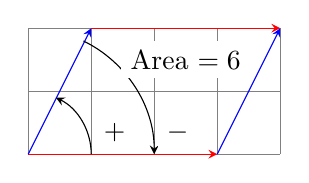
\begin{tikzpicture}[scale=.8]
\draw[help lines,step=1cm] (0,0) grid (4,2);
\draw[->,>=stealth,red] (0,0) -- (3,0);
\draw[->,>=stealth,red] [shift={(1,2)}](0,0) -- (3,0);
\draw[->,>=stealth,blue] (0,0) -- (1,2);
\draw[->,>=stealth,blue] [shift={(3,0)}](0,0) -- (1,2);
\draw[->,>=stealth] (0:1cm)  node[above right=1pt,fill=white]{\normalsize $+$} arc (0:64:1cm) ;
\draw[<-,>=stealth] (0:2cm)  node[above right=1pt,fill=white]{\normalsize $-$} arc (0:64:2cm) ;
\node[fill=white] at (2.5, 1.5) {Area $=6$}; 
\end{tikzpicture}

\vspace{2pt}
$\begin{vmatrix}{3}&{1}\\{0}&{2}\end{vmatrix}=6$ and $\begin{vmatrix}{1}&{3}\\{2}&0\end{vmatrix}=-6$
\end{center}
\caption{The determinant gives both area and direction. A counter clockwise rotation from column 1 to column 2 gives a positive determinant.\label{detfig}}
\end{figure}
%    }}

For a 3 by 3 matrix, the columns give the edges of a three dimensional parallelepiped and the determinant produces the volume of this object. The sign of the determinant is related to orientation. If you can use your right hand and place your index finger on the first vector, middle finger on the second vector, and thumb on the third vector, then the determinant is positive. 
For example, consider the matrix $A = \begin{bmatrix}\cl{1\\0\\0}&\cl{0\\2\\0}&\cl{0\\0\\3}\end{bmatrix}$.  Starting from the origin, each column represents an edge of the rectangular box 
$0\leq x\leq 1$, 
$0\leq y\leq 2$, 
$0\leq z\leq 3$ with volume (and determinant) $V=lwh=(1)(2)(3)=6$. The sign of the determinant is positive because if you place your index finger pointing in the direction (1,0,0) and your middle finger in the direction (0,2,0), then your thumb points upwards in the direction (0,0,3). 
If you interchange two of the columns, for example 
$B = \begin{bmatrix} \cl{0\\2\\0}&\cl{1\\0\\0}&\cl{0\\0\\3}\end{bmatrix}$, then the volume doesn't change since the shape is still the same. However, the sign of the determinant is negative because if you point your index finger in the direction (0,2,0) and your middle finger in the direction (1,0,0), then your thumb points down in the direction (0,0,-3). If you repeat this with your left hand instead of right hand, then your thumb points up.

\begin{problem}
\begin{itemize}
\item Use determinants to find the area of the triangle with vertices $(0,0)$, $(-2,5)$, and $(3,4)$.
\item What would you change if you wanted to find the area of the triangle with vertices $(-3,1)$, $(-2,5)$, and $(3,4)$? Find this area.
\end{itemize}
\end{problem}

\fi
%=========================================================
%End Matrix section that is not printed if Valpo is on.
%=========================================================
\section{Solving Systems of equations}


\begin{problem}
	\marginpar{For additional practice, make up your own systems of equations. Use \wolfA\  to check your work.}
		Solve the following linear systems of equations.
\begin{itemize}
\item $\begin{cases}x+y&=3\\2x-y&=4\end{cases}$
\item $\begin{cases}-x + 4y&=8\\3x - 12y&=2\end{cases}$
\end{itemize}
\end{problem}

\begin{problem}
	\marginpar{This 
		\href{http://www.wolframalpha.com/input/?i=Solve+x\%2B2y\%3D3+and+4x-y\%2Bz\%3D7+and+x\%3Dt}{link} 
		will show you how to specify which variable is $t$ when using Wolfram Alpha.}
Find all solutions to the linear system 
$\begin{cases}x+y+z&=3\\2x-y&=4\end{cases}$.  
Since there are more variables than equations, this suggests there is probably not just one solution, but perhaps infinitely many.  One common way to deal with solving such a system is to let one variable equal $t$, and then solve for the other variables in terms of $t$. Do this three different ways.
\begin{itemize}
\item If you let $x=t$, what are $y$ and $z$.  Write your solution in the form $(x,y,z)$ where you replace $x$, $y$, and $z$ with what they are in terms of $t$.
\item If you let $y=t$, what are $x$ and $z$ (in terms of $t$).
\item If you let $z=t$, what are $x$ and $y$.
\end{itemize}
\end{problem}


\newpage
\section{Optional: Higher Order Approximations} 
When you ask a calculator to tell you what $e^{.1}$ means, your calculator uses an extension of differentials to give you an approximation.  The calculator only uses polynomials (multiplication and addition) to give you an answer.  This same process is used to evaluate any function that is not a polynomial (so trig functions, square roots, inverse trig functions, logarithms, etc.) 
The key idea needed to approximate functions is illustrated by the next problem.

\begin{problem} 
Let $f(x)=e^x$. You should find that your work on each step can be reused to do the next step.
\begin{itemize}
\item Find a first degree polynomial $P_1(x)=a+bx$ so that $P_1(0)=f(0)$ and $P'_1(0)=f'(0)$. In other words, give me a line that passes through the same point and has the same slope as $f(x)=e^x$ does at $x=0$. Set up a system of equations and then find the unknowns $a$ and $b$. The next two are very similar.
\item Find a second degree polynomial $P_2(x)=a+bx+cx^2$ so that $P_2(0)=f(0)$, $P'_2(0)=f'(0)$, and $P''_2(0)=f''(0)$. In other words, give me a parabola that passes through the same point, has the same slope, and has the same concavity as $f(x)=e^x$ does at $x=0$. 
\item Find a third degree polynomial $P_3(x)=a+bx+cx^2+dx^3$ so that $P_3(0)=f(0)$, $P'_3(0)=f'(0)$, $P''_3(0)=f''(0)$, and $P'''_3(0)=f'''(0)$. In other words, give me a cubic that passes through the same point, has the same slope, the same concavity, and the same third derivative as $f(x)=e^x$ does at $x=0$. 
\item Now compute $e^{.1}$ with a calculator.  Then compute $P_1(.1)$, $P_2(.1)$, and $P_3(.1)$. How accurate are the line, parabola, and cubic in approximating $e^{.1}$?
\end{itemize}
\end{problem} 



\begin{problem} 
	\marginpar{The polynomial you are creating is often called a Taylor polynomial. (I'm giving you the name so that you can search online for more information if you are interested.)}
Now let $f(x)=\sin x$. Find a 7th degree polynomial so that the function and the polynomial have the same value and same first seven derivatives when evaluated at $x=0$. Evaluate the polynomial at $x=0.3$. How close is this value to your calculator's estimate of $\sin(0.3)$?  You may find it valuable to use the notation $$P(x) = a_0+a_1x+a_2x^2+a_3x^3 +\cdots+a_7 x^7.$$
\end{problem}




The previous two problems involved finding polynomial approximations to the function at $x=0$. The next problem shows how to move this to any other point, such as $x=1$. 
\begin{problem} \label{Taylor at 1}
Let $f(x)=e^x$.
\begin{itemize}
\item Find a second degree polynomial $$T(x)=a+bx+cx^2$$ so that $T(1)=f(1)$, $T'(1)=f'(1)$, and $T''(1)=f''(1)$. In other words, give me a parabola that passes through the same point, has the same slope, and the same concavity as $f(x)=e^x$ does at $x=1$. 
\item Find a second degree polynomial written in the form $$S(x)=a+b(x-1)+c(x-1)^2$$ 
	\marginpar{Notice that we just replaced $x$ with $x-1$. This centers, or shifts, the approximation to be at $x=1$. The first part will be much simpler now when you let $x=1$.} so that $S(1)=f(1)$, $S'(1)=f'(1)$, and $S''(1)=f''(1)$. In other words, find a quadratric that passes through the same point, has the same slope, and the same concavity as $f(x)=e^x$ does at $x=1$. 
\item Find a third degree polynomial written in the form $$P(x)=a+b(x-1)+c(x-1)^2+d(x-1)^3$$ so that $P(1)=f(1)$, $P'(1)=f'(1)$, $P''(1)=f''(1)$, and $P'''(1)=f'''(1)$. In other words, give me a cubic that passes through the same point, has the same slope, the same concavity, and the same third derivative as $f(x)=e^x$ does at $x=1$. 
\end{itemize}
\end{problem} 


%The problems above introduced the final idea. We will let $dx=x-c$ (a small change in $x$). Since the polynomial should be close to the function, a small change in $y$ is $dy=P_n(x)-f(c)$. We can write the Taylor polynomial notation above in the form  
% $$P_n(x) - f(c)=dy=\frac{f'(c)}{1!}dx+\frac{f''(c)}{2!}dx^2+\cdots +\frac{f^{(n)}(c)}{n!}dx^n. $$
% If we want to estimate the change in $y$ using a first order approximation, this gives us the differential notation
% $$dy = f'(c)dx.$$
% A second order approximation is
% $$dy = f'(c)dx + \frac{f''(c)}{2!}dx^2.$$
% A third order approximation is
% $$dy = f'(c)dx + \frac{f''(c)}{2!}dx^2+  \frac{f'''(c)}{3!}dx^3.$$
 

\begin{example}
This example refers back to problem \ref{diff-sphere}. We wanted a spherical tank of radius 3m, but due to manufacturing error the radius was slightly off. Let's now illustrate how we can use polynomials to give a first, second, and third order approximation of the volume if the radius is 3.02m instead of 3m.  

We start with $V=\frac{4}{3} \pi r^3$ and then compute the derivatives $$V'=4\pi r^2, V''=8\pi r, \text{ and } V'''=8\pi.$$ Because we are approximating the increase in volume from $r=3$ to something new, we'll create our polynomial approximations centered at $r=3$. We'll consider the polynomial 
$$P(r)=a_0+a_1(r-3)+a_2(r-3)^2+a_3(r-3)^3,$$ 
whose derivatives are 
$$P'=a_1+2a_2(r-3)+3a_3(r-3)^2,
P''=2a_2+6a_3(r-3),
P'''=6a_3.$$
So that the derivatives of the volume function match the derivatives of the polynomial (at $r=3$), we need to satisfy the equations in the table below.
\begin{center}
\begin{tabular}{|c|c|c|c|}\hline
 $k$ & Value of $V$ at the $k$th derivative & Value of $P$ at the the $k$th derivative & Equation \\ \hline
 $0$ & $V(3) = \frac{4}{3}\pi (3)^3 = 36\pi$ & $P(3) = a_0$ & $a_0=36\pi$ \\ \hline
 $1$ & $V'(3) = 4\pi (3)^2=36\pi$ & $P'(3) = a_1$ & $a_1=36\pi$ \\ \hline
 $2$ & $V''(3) = 8\pi (3)=24\pi$ & $P''(3) = 2a_2$ & $2a_2=24\pi$ \\ \hline
 $3$ & $V'''(3) = 8\pi$ & $P'''(3) = 6a_3$ & $6a_3=8\pi$ \\ \hline
\end{tabular}
\end{center}
This tells us that the third order polynomial is 
$$P(r)=a_0+a_1(r-3)+a_2(r-3)^2+a_3(r-3)^3
=36\pi+36\pi(r-3)+12\pi(r-3)^2+\frac{4}{3}\pi(r-3)^3
.$$ 
We wanted to approximate the volume if $r=3.2$, so our change in $r$ is $dr=3.2-3=0.2$.  We can rewrite our polynomial as
$$P(r)=36\pi+36\pi(dr)+12\pi(dr)^2+\frac{4}{3}\pi(dr)^3.$$
We are now prepared to approximate the volume using a first, second, and third order approximation. 
 \begin{enumerate}
 \item A first order approximation yields $P=36\pi+ 36\pi\cdot 0.02 =36.72\pi.$ The volume increased by $0.72\pi$ m$^3$. 
 \item A second order approximation yields $$P=36\pi+ 36\pi\cdot 0.02 +12\pi (0.02)^2 =36.7248\pi.$$
 \item A third order approximation yields $$P=36\pi+36\pi\cdot 0.02 +12\pi (0.02)^2+\frac{4}{3}\pi(0.02)^3  =36.724810\bar6\pi.$$
 \end{enumerate}
With each approximation, we add on a little more volume to get closer to the actual volume of a sphere with radius $r=3.02$. The actual volume of a sphere involves a cubic function, so when we approximate the volume with a cubic, we should get an exact approximation (and $ V(3.02) = \frac 43 \pi (3.02)^3 =(36.724810\bar6)\pi$.)
 \end{example}
 
 We'll end this section with a problem to practice the example above.
 
 \begin{problem}
 Suppose you are constructing a cube whose side length should be $s=2$ units. The manufacturing process is not exact, but instead creates a cube with side lengths $s=2+ds$ units. (You should assume that all sides are still the same, so any error on one side is replicated on all.  We have to assume this for now, but before the semester ends we'll be able to do this with high dimensional calculus.) 
 
 \marginpar{As a challenge, try to draw a 3D graph which illustrates the volume added on by each successive approximation. If you have it before we get here as a class, let me know and I'll let you share what you have discovered with the class.} Suppose that the machine creates a cube with side length $2.3$ units instead of 2 units.  Note that the volume of the cube is $V=s^3$.  Use a first, second, and third order approximation to estimate the increase in volume caused by the .3 increase in side length.  Then compute the actual increase in volume $V(2.3)-V(2)$.   
 \end{problem}
\note{I would include this problem above in class as a demonstration.  It allows them to see what differentials do.  You can easily see how each new piece adds more to the approximation.}

%\section{Wrap Up}
%This concludes the chapter.  Look at the objectives at the beginning of the chapter. Can you now do all the things you were promised? \\
%\textbf{Lesson Plan Creation\\}
%Your assignment: organize what you've learned into a small collection of examples that illustrates the key concepts. I'll call this your one-page lesson plan. You may use both sides. The objectives at the beginning of the chapter give you a list of the key concepts. Once you finish your lesson plan, scan it into a PDF document (use any scanner on campus), and then upload the document to Blackboard.
%
%As you create this lesson plan, consider the following:
%\begin{itemize}
 %\item On the class period after making this plan, you'll have 20 minutes in class where you will get to teach a peer your examples. If you keep the examples simple, you'll be able to fully review the entire chapter.\\
%\textbf{Note: For this review chapter only, we will NOT have a 20 minute in-class session}
 %\item Before each celebration of knowledge we will devote a class period to review. With well created lesson plans, you will have 4-8 (for 2-4 Chapters) to review for each, instead of 50-100 problems.
 %\item Think ahead 2-5 years. If you make these lesson plans correctly, you'll be able to look back at your lesson plans for this semester. In about 10 pages, you can have the entire course summarized and easy for you to recall.
%\end{itemize}


\clearpage
%%% Local Variables: 
%%% mode: latex
%%% TeX-master: "215-problems"
%%% End: 
